\chapter{Konzeption der Anwendung}
\label{chapter:Konzeption der Anwendung}

In diesem Kapitel wird die Konzeption der Anwendung beschrieben. Zunächst wird die Grundidee vorgestellt. Anschließend wird ein genaues technologisches Konzept erstellt.

\section{Grundidee} %Benedikt
\label{section:Grundidee} %Benedikt
Bekannte Zusammenhänge zwischen prognostiziertem und tatsächlichem Wert sind meist durch einfache Rechenoperationen umsetzbar. So kann beispielsweise eine Erhöhung der Mehrwertsteuer für ein Produktpreis P mit einer Rechenoperation P = P * M errechnet werden. Für diese Zusammenhänge ist es meist nicht notwendig und sinnvoll, komplexe und vernetzte Softwaresysteme zu entwickeln. 

Wie anfangs erwähnt wird bei Börsenprognosen versucht, \emph{nicht-lineare Zusammenhänge} innerhalb von Daten zu finden, da lineare und bekannte Zusammenhänge, die zudem noch exakt sind quasi nicht vorhanden sind. Deshalb ist es für die Anwendung sinnvoll und notwendig einen komplexeren und vernetzeren Ansatz zu verfolgen, auch wenn dies mit einer Steigerung der Kosten einher geht. 

Neben dem Hauptziel, die Zeitreihenextrapolation von Börsendaten, soll gezeigt werden, wie es konzeptionell und technisch möglich ist, eine derartige Softcomputing-Lösung zu realisieren und in einen Unternehmenskontext zu integrieren.

Weitere Faktoren, die bei der Entscheidung über die eingesetzten Frameworks und Werkzeuge mit eingeflossen sind, sind Skalierbarkeit, Wartbarkeit, Erreichbarkeit sowie Anschaulichkeit. 

\begin{minipage}[c]{0.5\textwidth}

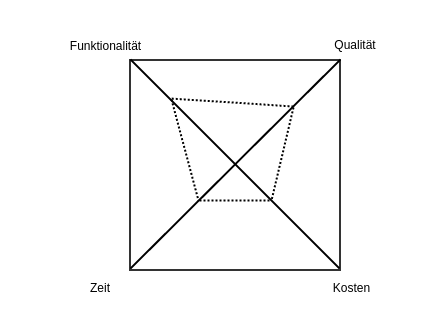
\includegraphics[width=0.49\textwidth]{Bilder/Konzeption/mag_viereck_not_linear.png}
\captionof{figure}{Abb - nicht lineare}

\end{minipage}
\begin{minipage}[c]{0.5\textwidth}
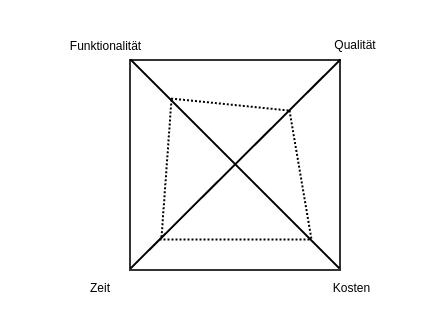
\includegraphics[width=0.49\textwidth]{Bilder/Konzeption/mag_viereck_linear.png}
\captionof{figure}{Abb - lineare}
\end{minipage}

\paragraph{Quandl Data-Provider}
Für Börenprognosen werden quantitative Maßeinheiten benötigt, die im Zusammenhang mit Kurs stehen. Die Wohl aussagekräftigste sind Börsenschluss-Index-Werte von vergangenen Handelsperioden. Je mehr dieser Daten vorhanden, je realistischer diese Daten sind, desto warscheinlicher ist es, einen Schlusswert in der Zukunft vorherzusagen. 
Aus diesem Grund spricht die Anwendung, genauer der Rest-Controller der Stockmarket-Webapp den Rest-Service von Quandl an.  
Quandl versteht sich als Datenhändler / Datenanbieter mit integrierter Suchfunktion. Das Angebot umfasst die globale Finanzbranche, so z.B. sämtliche nationale und internationale Börsenkurse der vergangenen Dekaden. 
Die Rest-API bietet die Export-Formate \emph{XML}, \emph{JSON} und \emph{CSV} an.\linebreak; 
Diese ermöglicht der Anwendung mit echten Börsendaten zu arbeiten. 

[https://www.quandl.com/blog/getting-started-with-the-quandl-api].\linebreak;

\paragraph{Stockmarket-Webapp}
Bei der Stockmarket-Webapp handelt es sich um einen Restful-Service der als Schnittstelle zwischen der Quandl-Rest-API, der Visualisierung sowie dem Neuroph Werkzeug fungiert. Wie in Abbildung ABBILDUNG zu sehen ist gibt es keine Kommunikation zwischen Fremd-Services, wenn diese nicht über den Controller der Stockmarket-Webapp statt findet. Hierüber können gleich mehrere Vorteile realisiert werden. 
1) Single-Point-Of-Failure: Wenn der Datenlieferant Quandl insolvent geht oder nicht ganz so drastisch, wenn die Anfrage-Mechanismen der Quandl-Rest-API geändert werden. Ein weiteres Szenario, könnte aus Sicht der Visualisierung einen aus Performance-Bedingten Wechsel der JavaScript-Bibliothek darstellen. Sofern für diese Szenarien keine SPOF-Lösung existiert, wird eine entsprechende Anpassung womöglich ein umfassendes Refactoring aller Anwendungskoponenten erfordern. 
2) Skalierbarkeit: Den Fall angenommen, weitere Datensätze sollen an andere Visualisierungen bzw. die Visualisierung um Diagramme erweitert werden, so ist bereits mit einer einseitigen Anpassung der Visualisierung die Anforderung erfüllt. Die durch die Rest-Spezifikation definierte Tatsache der einheitlichen Repräsentation von Anfragen spielt einem hier in die Hände. \\
Die Aufgabe der Stockmarket-Webapp ist es eine schnittstellen - und benutzerdefinierte Datenaufbereitung zu realisieren. 

\paragraph{Visualisierung}
Die Grundidee die Visualisierung von der Anwendungslogik weitgehend zu trennen hat diverse Vorteile. Die Abhängigkeitsreduktion von anderen Komponenten, sowie Sicherheitsaspekte spielen dabei eine besondere Rolle. 
Die Visualisierung ist eine rein Client-seitig laufende Anwendung. Diese enthält alle notwendigen Logikroutinen, um Daten anzufragen und entsprechend zu verarbeiten. Die Implementierung dieser Logik wird mit der JavaScript-Bibliothek jQuery umgesetzt. Diese speißt und manipuliert das Document-Object-Model(DOM) je nach \emph{Datenlage}. Das DOM kann auch als HTML-Gerüst bezeichnet werden. Für die visuellen Effekte, die eine bessere Veranschaulichung der Graphen ermöglichen soll, wird CSS eingesetzt. Um das Layout für Geräte mit unterschiedlicher Displaygröße gleichermaßen nutzbar zu machen, wird die CSS-Bibliothek Bootstrap verwendet. 

\begin{figure}
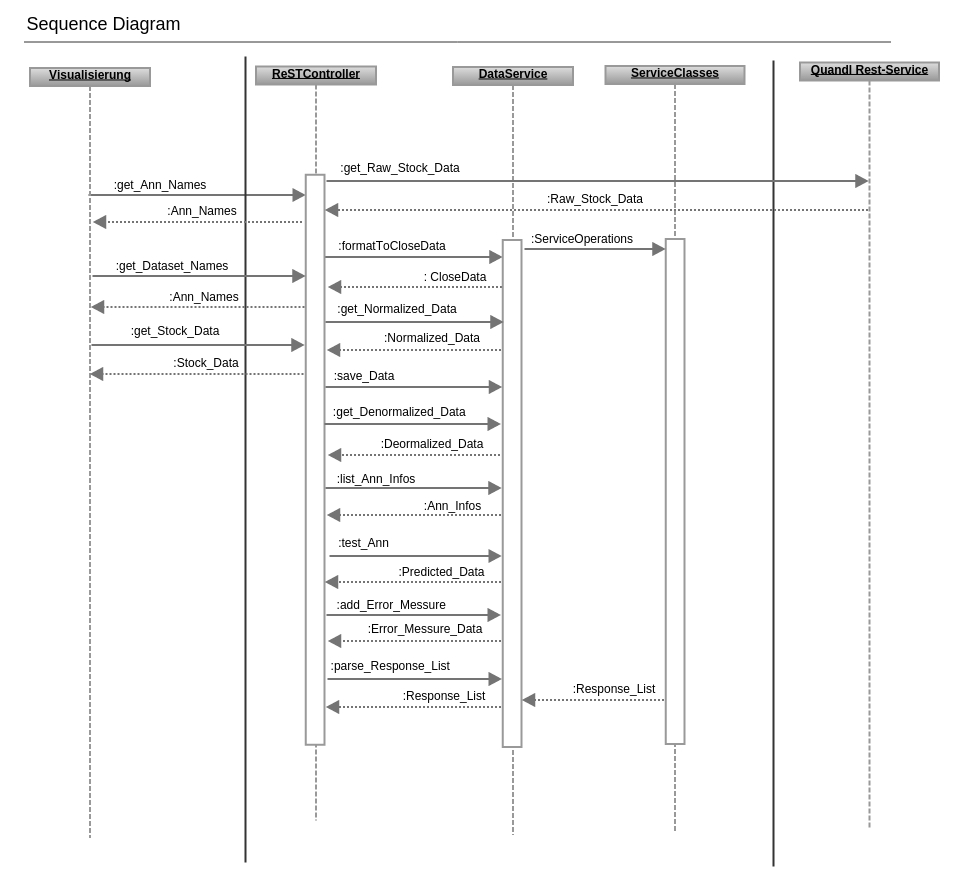
\includegraphics[width=15cm]{Bilder/Konzeption/sequence_dia_rest_env.png}
\captionof{figure}{Sequenzdiagramm}
\end{figure}


\section{Technologie}
\label{section:Technologie}

\subsubsection{Rest-Kommunikation}
Die Kommunikation zwischen den drei konzeptionell festgelegten Komponenten soll ausschließlich über das Programmierparadigma von ReST (Representational State Transfer) von statten gehen. Damit eine Kommunikation als \emph{Restful} bezeichnet werden kann müssen einige Kriterien erfüllt werden. Ein Rest-Service ist adressierbar, jeder Rest-Endpunkt hat eine eindeutige URI. Das Format der zurückgelieferten Ressource kann variieren. So können beispielsweise \emph{CSV}, \emph{HTML}, \emph{XML} und \emph{JSON} gleichermaßen von einem Rest-Service geliefert werden. Hierbei ist das Prinzip der Zustandslosigkeit zu beachten, also egal in welchem Format ein Nachricht ankommt, der Informationsgehalt muss äquivalent für gleiche Anfragen sein. Der Kommunikationskanal ist zwar nicht festgeschrieben, ist aber ich aller Regel das HTTP. Hierbei gilt es die entsprechenden Empfehlungen für die HTTP-Verbs zu beachten. Dies ist vor allem im Punkt Sicherheit wichtig.   

\subsection{Frameworks}
Zu den nachfolgenden Frameworks und Bibliotheken werden hauptsächlich anwendungsrelevante Funktionalitäten erläutert, da es sonst den Rahmen dieser Seminararbeit sprengen würde.

\paragraph{Spring Boot}
Spring ist ein unter der Apache Lizenz veröffenlichtes, quelloffenes Java-Framework. Eine umfassende Übersicht würde den Rahmen dieser Seminararbeit sprengen. Daher wird im folgenden auf auf zwei besonders markante und wichtige Punkte kurz eingegangen. Beide Verfahren zielen darauf ab, Wiederholungen im Quellcode zu vermeiden sowie insgesamt prägnatere Anweisungen umzusetzen. Diese Thematik wird unter dem Begriff des \emph{Boilerplate Code} oder besser die Vermeidung von Boilerplate Code geführt. Spring Boot bietet eine vereinfachte und schnellere Möglichkeit Anwendungen zu entwickeln, da noch vielfältigere Art und Weise Abhängigkeiten integriert werden können, so kann z.B. ein Tomcat-Server automatisch eingebunden werden.  

\paragraph{Dependency Injection}
Die Abhängigkeitsinjektion zielt darauf ab, möglichst wenig Abhängigkeiten zwischen Java-Klassen zu konstruieren. Dependency Injection ist ein Entwurfsmuster (Software Pattern) das dieses umsetzt. Instanzen von Javaklassen müssen demnach ihre Abhängigkeitsinformationen durch einen Aufruf von Methoden einer externen Instanz zugewiesen bekommen. Deshalb wird dieser Vorgang als Injektion bezeichnet. Es werden drei verschiedene Arten von Abhängigkeitsinjektionen unterschieden, die \emph{Inversion of Control} (IoC), die Konstruktorinjektion sowie die Setterinjektion. Spring implementiert beispielsweise einen sogenannten IoC-Container. Die darin enthaltenen Objekte verweisen explizit auf Abhängigkeiten, woraus sogenannte Java-Beans (Klassen die der Spezifikation LINK genügen) konstruiert werden. Spring bemüht sich im Grund darum  \emph{Best-Pratices} der Softwareentwicklung im Javaumfeld umzusetzen und den Entwickler hierbei zu unterstützen. Nähers zum Thema Spring kann z.B. unter dem LINK nachgelesen werden.


\subsection{Annotationen}
Annotationen sind äußerlich leicht zu erkennen. Sie beginnen mit einem \emph{@}-Zeichen und können Methoden sowie Klassen gleichermaßen kennzeichnen. Annotationen sind Schnittstellen (Interfaces), die grob in zwei Arten unterteilt werden können. Zum einen diejenigen die während der Kompilierzeit ausgeführt werden und anschließend nicht mehr benötigt werden wie beispielsweise die \emph{@Override}-Annotation für die Implementierung von Methoden abstrakter Klassen. Die zweite Art ist auch während der Laufzeit noch von Bedeutung, so z.B. die \emph{@Autowired}-Annotation. Diese gibt explizit an, dass eine Klasse per Dependency-Injection in die Programmlogik integriert werden soll. 

\paragraph{Javascript Bibliothek - C3js}
Die Auswahl einer geeigneten Javascript-Bibliothek ist nicht leicht. Es gibt zahlreiche gut umgesetzte Lösungen im Umlauf, welche in unterschiedliche Bereichen jeweils Vor - und Nachteile bieten. \emph{C3js} ist eine relativ schlank und verzichtet auf einige Zusatzkomponenten. Die Basis für C3 ist die \emph{D3js} Bibliothek, deren Diagramme meist einen höheren Grad an visuellen Extravaganzen umsetzt oder auf spezielle Einsatzgebiete eingeht. D3js eignet sich daher eher für ausgefallenere Diagramme, C3 wurde aus Performance-Gründen gewählt und weil die angebotenen Funktionen den gewünschten Informationsgehalt entsprechend darstellen kann.   

\paragraph{Layouts und CSS Bootstrap}
Das Bootstrap Framework ist eine freie und sehr umfangreiche Bibliothek, die Komponenten und Funktionalitäten bereitstellt, die sich an den neuesten Webdesign-Kriterien orientiert. Sie wird unter der MIT-Lizenz veröffentlicht und unterstützt die am bekanntesten Browser. Die Visualisierung profitiert start von der Möglichkeit, das HTML-Gerüst dynamisch an verschiedene Displaygrößen anzupassen (Responsive Design). 

\subsection{Apache Maven}
Die benötigten Frameworks können auf verschiedene Wege eingebunden werden. Die Softwarepakete können per Hand heruntergeladen und in den entsprechenden Verzeichnispfad kopiert werden, was allerdings bei größeren Projekten hinsichtlicher der Übersicht und Verwaltbarkeit problematisch ist. Ein besserer Ansatz ist es ein Build-Tool wie Apache Maven zu verwenden, was auch für diese Anwendung eingesetzt wurde. Alternative Build-Tools sind z.B. Apache Ant und Gradle.\\
Zentraler Beschreibungspunkt, der das Projekt benötigter Abhängigkeiten und Build-Prozesse ist die POM.xml. POM steht dabei für \emph{Projekt Object Model}.
Die Softwarepakte heißten im Maven-Jargon \emph{Dependencies}, also Abhängigkeiten. Dependencies werden in \emph{Repositories} verwaltet. Es gibt zwei Arten, \emph{local} und \emph{remote} Repositories.   
Die lokale Datenhaltungskomponente stellt eine exakte Kopie aller heruntergeladenen Dependencies sowie deren Verzeichnisstruktur, von rechnerfernen Repositories dar. 
